\documentclass[11pt]{article}
\usepackage[english]{babel}
\usepackage[utf8]{inputenc}
\usepackage{physics}
\usepackage{caption}
\usepackage{subcaption}
\usepackage{qcircuit}
\usepackage{amsmath,amssymb,graphicx}
\usepackage{mathtools}
\usepackage{geometry}
\usepackage{booktabs}
\usepackage{hyperref}
\usepackage{enumitem}
\geometry{a4paper, margin=1in}
\setlength{\parskip}{0.8em}
\setlength{\parindent}{0pt}

\title{FYS5419 Project 1\\[0.3em] Variational Quantum Eigensolver for the Lipkin Model}
\author{Aleksander N.\ Sekkelsten\\
        \small Faculty of Mathematics and Natural Sciences, University of Oslo}
\date{March 2026}

\begin{document}
\maketitle

\begin{abstract}
We implement the Variational Quantum Eigensolver (VQE) algorithm using pure matrix simulation (NumPy/SciPy) and apply it to the Lipkin model, a simplified many-body quantum system from nuclear physics. Starting from single-qubit operations, Bell state entanglement, and simple Hamiltonian eigenproblems, we build up to VQE simulations of progressively larger systems: a one-qubit Hamiltonian (2D), a two-qubit Hamiltonian (4D), and the Lipkin Hamiltonian for $J=1$ (3D) and $J=2$ (5D). The VQE ground state energies agree with exact diagonalization to within $10^{-6}$ for $J=1$ and $10^{-4}$ for $J=2$ across the full range of interaction strengths. We also analyze the entanglement structure of the ground state through von Neumann entropy, demonstrating how interactions drive quantum correlations.
\end{abstract}

%======================================================================
\section{Introduction}
%======================================================================

The Variational Quantum Eigensolver (VQE)~\cite{Peruzzo2014} is a hybrid quantum--classical algorithm for estimating the ground state energy of a Hamiltonian. A parameterized quantum state (ansatz) $\ket{\psi(\boldsymbol\theta)}$ is prepared on a quantum device, and the expectation value $\bra{\psi(\boldsymbol\theta)} H \ket{\psi(\boldsymbol\theta)}$ is measured. A classical optimizer then updates the parameters $\boldsymbol\theta$ to minimize this energy, exploiting the variational principle $E_{\text{VQE}} \geq E_0$.

The Lipkin model~\cite{Lipkin1965} has long served as a testbed for many-body methods because it captures essential features of interacting quantum systems---collective excitations, symmetry breaking, and entanglement transitions---while remaining analytically tractable. In this project we apply VQE to the Lipkin model for total spins $J=1$ (two particles) and $J=2$ (four particles), constructing appropriate variational ans\"atze and comparing with exact diagonalization.

All computations are performed with pure matrix simulation using NumPy and SciPy---no external quantum computing frameworks (Qiskit, Pennylane, etc.) are used. The codebase is organized into a modular \texttt{src/} package with separate modules for gates, states, measurements, entropy, Hamiltonians, VQE, and plotting. A Jupyter notebook (\texttt{main.ipynb}) runs all computations and generates all figures.

%======================================================================
\section{Part a: Single-Qubit Operations, Bell States, and Entanglement}
%======================================================================

\subsection{Single-qubit gates}

We define the computational basis $\ket{0} = (1, 0)^T$, $\ket{1} = (0, 1)^T$ and verify the action of the standard gates ($X, Y, Z, H, S$). Table~\ref{tab:gates} summarizes the outputs.

\begin{table}[h!]
\centering
\begin{tabular}{@{}llll@{}}
\toprule
\textbf{Gate} & \textbf{Matrix} & $\textbf{Gate}\ket{0}$ & $\textbf{Gate}\ket{1}$ \\ \midrule
$X$ & $\begin{psmallmatrix}0&1\\1&0\end{psmallmatrix}$ & $\ket{1}$ & $\ket{0}$ \\[4pt]
$Y$ & $\begin{psmallmatrix}0&-i\\i&0\end{psmallmatrix}$ & $i\ket{1}$ & $-i\ket{0}$ \\[4pt]
$Z$ & $\begin{psmallmatrix}1&0\\0&-1\end{psmallmatrix}$ & $\ket{0}$ & $-\ket{1}$ \\[4pt]
$H$ & $\frac{1}{\sqrt{2}}\begin{psmallmatrix}1&1\\1&-1\end{psmallmatrix}$ & $\ket{+}$ & $\ket{-}$ \\[4pt]
$S$ & $\begin{psmallmatrix}1&0\\0&i\end{psmallmatrix}$ & $\ket{0}$ & $i\ket{1}$ \\ \bottomrule
\end{tabular}
\caption{Actions of single-qubit gates on the computational basis states.}
\label{tab:gates}
\end{table}

\subsection{Bell states}

The four Bell states form a maximally entangled basis for two qubits:
\begin{align}
\ket{\Phi^\pm} &= \frac{1}{\sqrt{2}}(\ket{00} \pm \ket{11}), &
\ket{\Psi^\pm} &= \frac{1}{\sqrt{2}}(\ket{01} \pm \ket{10}).
\end{align}
$\ket{\Phi^+}$ is created from $\ket{00}$ via $H \otimes I$ followed by CNOT:
\[
\ket{00} \xrightarrow{H \otimes I} \frac{1}{\sqrt{2}}(\ket{0}+\ket{1})\ket{0} \xrightarrow{\text{CNOT}} \frac{1}{\sqrt{2}}(\ket{00}+\ket{11}).
\]

\subsection{Measurements and correlations}

Measuring $\ket{\Phi^+}$ in the computational basis yields $\ket{00}$ and $\ket{11}$ each with probability $1/2$. We verify:
\begin{itemize}[nosep]
  \item $\expval{Z_0} \approx 0$, $\expval{Z_1} \approx 0$ (each qubit individually random),
  \item $\expval{Z_0 Z_1} = 1$ (perfectly correlated).
\end{itemize}
Applying the inverse Bell circuit (CNOT then $H \otimes I$) decodes $\ket{\Phi^+}$ back to $\ket{00}$ deterministically, confirmed by 50\,000 shots.

\subsection{Von Neumann entropy}

For a Bell state, the reduced density matrix of subsystem $A$ is $\rho_A = \frac{1}{2}I$, giving the maximum single-qubit entropy:
\[
S(\rho_A) = -\tr(\rho_A \log_2 \rho_A) = -2 \cdot \frac{1}{2}\log_2 \frac{1}{2} = 1~\text{bit}.
\]
We verify that all four Bell states have $S = 1$ bit, while the product state $\ket{00}$ has $S = 0$. This confirms that Bell states are \emph{maximally entangled}.

%======================================================================
\section{Part b: One-Qubit Eigenvalue Problem}
%======================================================================

We define $H = H_0 + \lambda H_I$ with:
\[
H_0 = \mathcal{E}\, I + \Omega\, \sigma_z, \qquad H_I = c\, I + \omega_z\, \sigma_z + \omega_x\, \sigma_x
\]
where $E_1 = 0$, $E_2 = 4$, $V_{11} = 3$, $V_{22} = -3$, $V_{12} = 0.2$. This gives $\mathcal{E} = 2$, $\Omega = -2$, $c = 0$, $\omega_z = 3$, $\omega_x = 0.2$, so:
\[
H(\lambda) = \begin{pmatrix} 3\lambda & 0.2\lambda \\ 0.2\lambda & 4 - 3\lambda \end{pmatrix}.
\]
The eigenvalues are:
\[
E_\pm = 2 \pm \frac{1}{2}\sqrt{(6\lambda - 4)^2 + 0.16\lambda^2}.
\]

At $\lambda = 2/3$ the diagonal elements are equal, producing an \emph{avoided crossing}. For $\lambda < 2/3$ the ground state is dominated by $\ket{0}$; for $\lambda > 2/3$ it shifts toward $\ket{1}$. Figure~\ref{fig:part_b} shows the eigenvalue spectrum and the ground state composition as a function of $\lambda$.

\begin{figure}[h!]
\centering
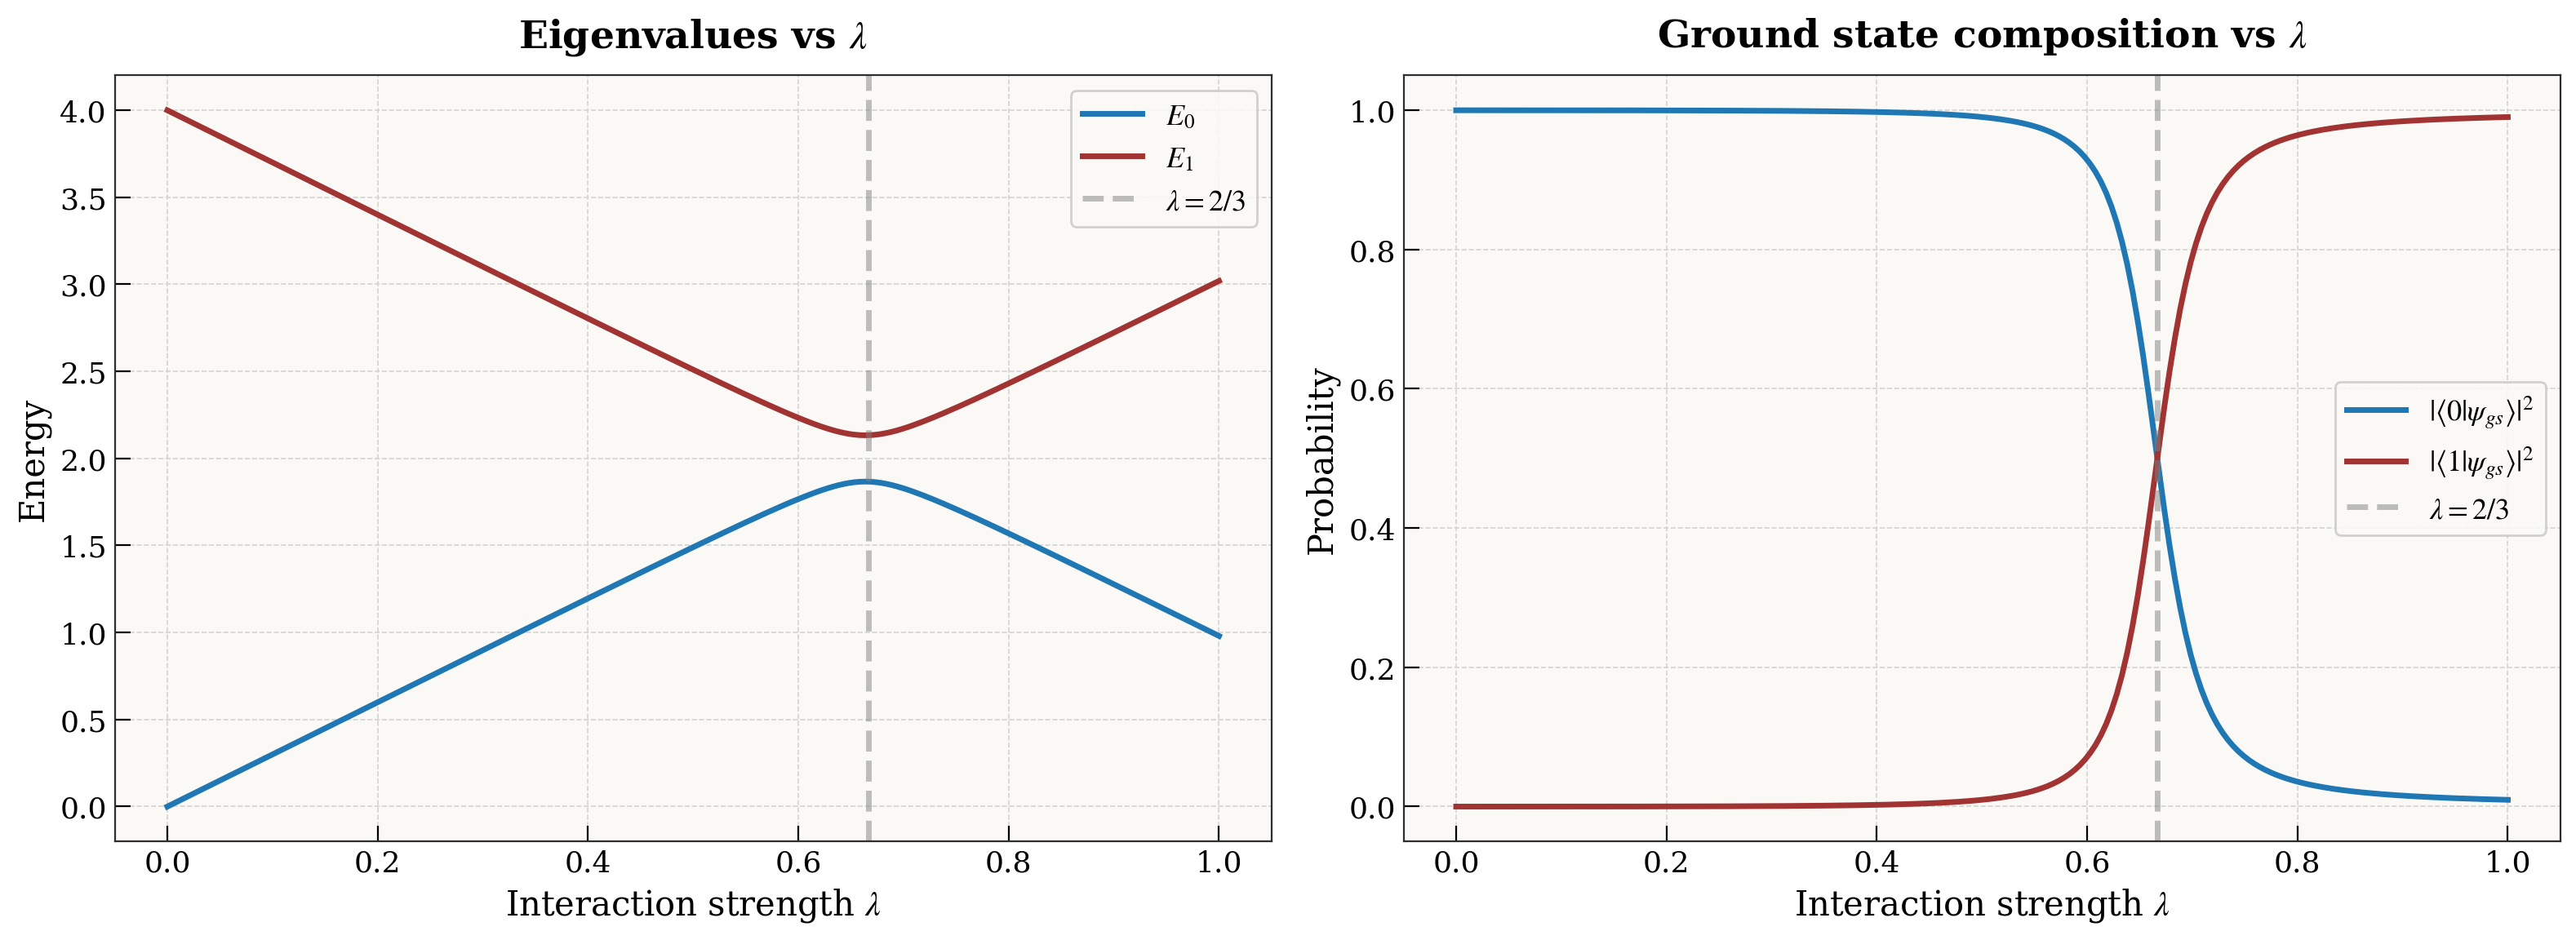
\includegraphics[width=0.85\linewidth]{images/part_b_eigenvalues.png}
\caption{Part b: Eigenvalues (left) and ground state composition (right) vs.\ interaction strength $\lambda$ for the one-qubit Hamiltonian. The avoided crossing at $\lambda = 2/3$ is marked with a dashed line.}
\label{fig:part_b}
\end{figure}

%======================================================================
\section{Part c: VQE for the One-Qubit System}
%======================================================================

\subsection{Ansatz}

We parameterize a general single-qubit state:
\[
\ket{\psi(\theta, \phi)} = \cos\frac{\theta}{2}\ket{0} + e^{i\phi}\sin\frac{\theta}{2}\ket{1},
\]
equivalent to applying $U_3(\theta, \phi, 0)$ to $\ket{0}$. Since this spans the full Bloch sphere, it can represent any single-qubit pure state.

\subsection{Pauli decomposition}

The Hamiltonian is already expressed in Pauli form: $H(\lambda) = (\mathcal{E} + \lambda c)I + (\Omega + \lambda\omega_z)\sigma_z + \lambda\omega_x\sigma_x$. The expectation value is:
\[
\expval{E} = (\mathcal{E} + \lambda c) + (\Omega + \lambda\omega_z)\expval{\sigma_z} + \lambda\omega_x\expval{\sigma_x}
\]
where $\expval{\sigma_z} = \cos\theta$ and $\expval{\sigma_x} = \sin\theta\cos\phi$. The COBYLA optimizer minimizes this over $(\theta, \phi)$.

\subsection{Results}

Figure~\ref{fig:part_c} shows the VQE energy closely matching the exact diagonalization across the full range of $\lambda$, with errors below $10^{-5}$. This is expected: the ansatz spans the complete 2D Hilbert space, so the optimizer always finds the exact ground state (up to numerical precision).

\begin{figure}[h!]
\centering
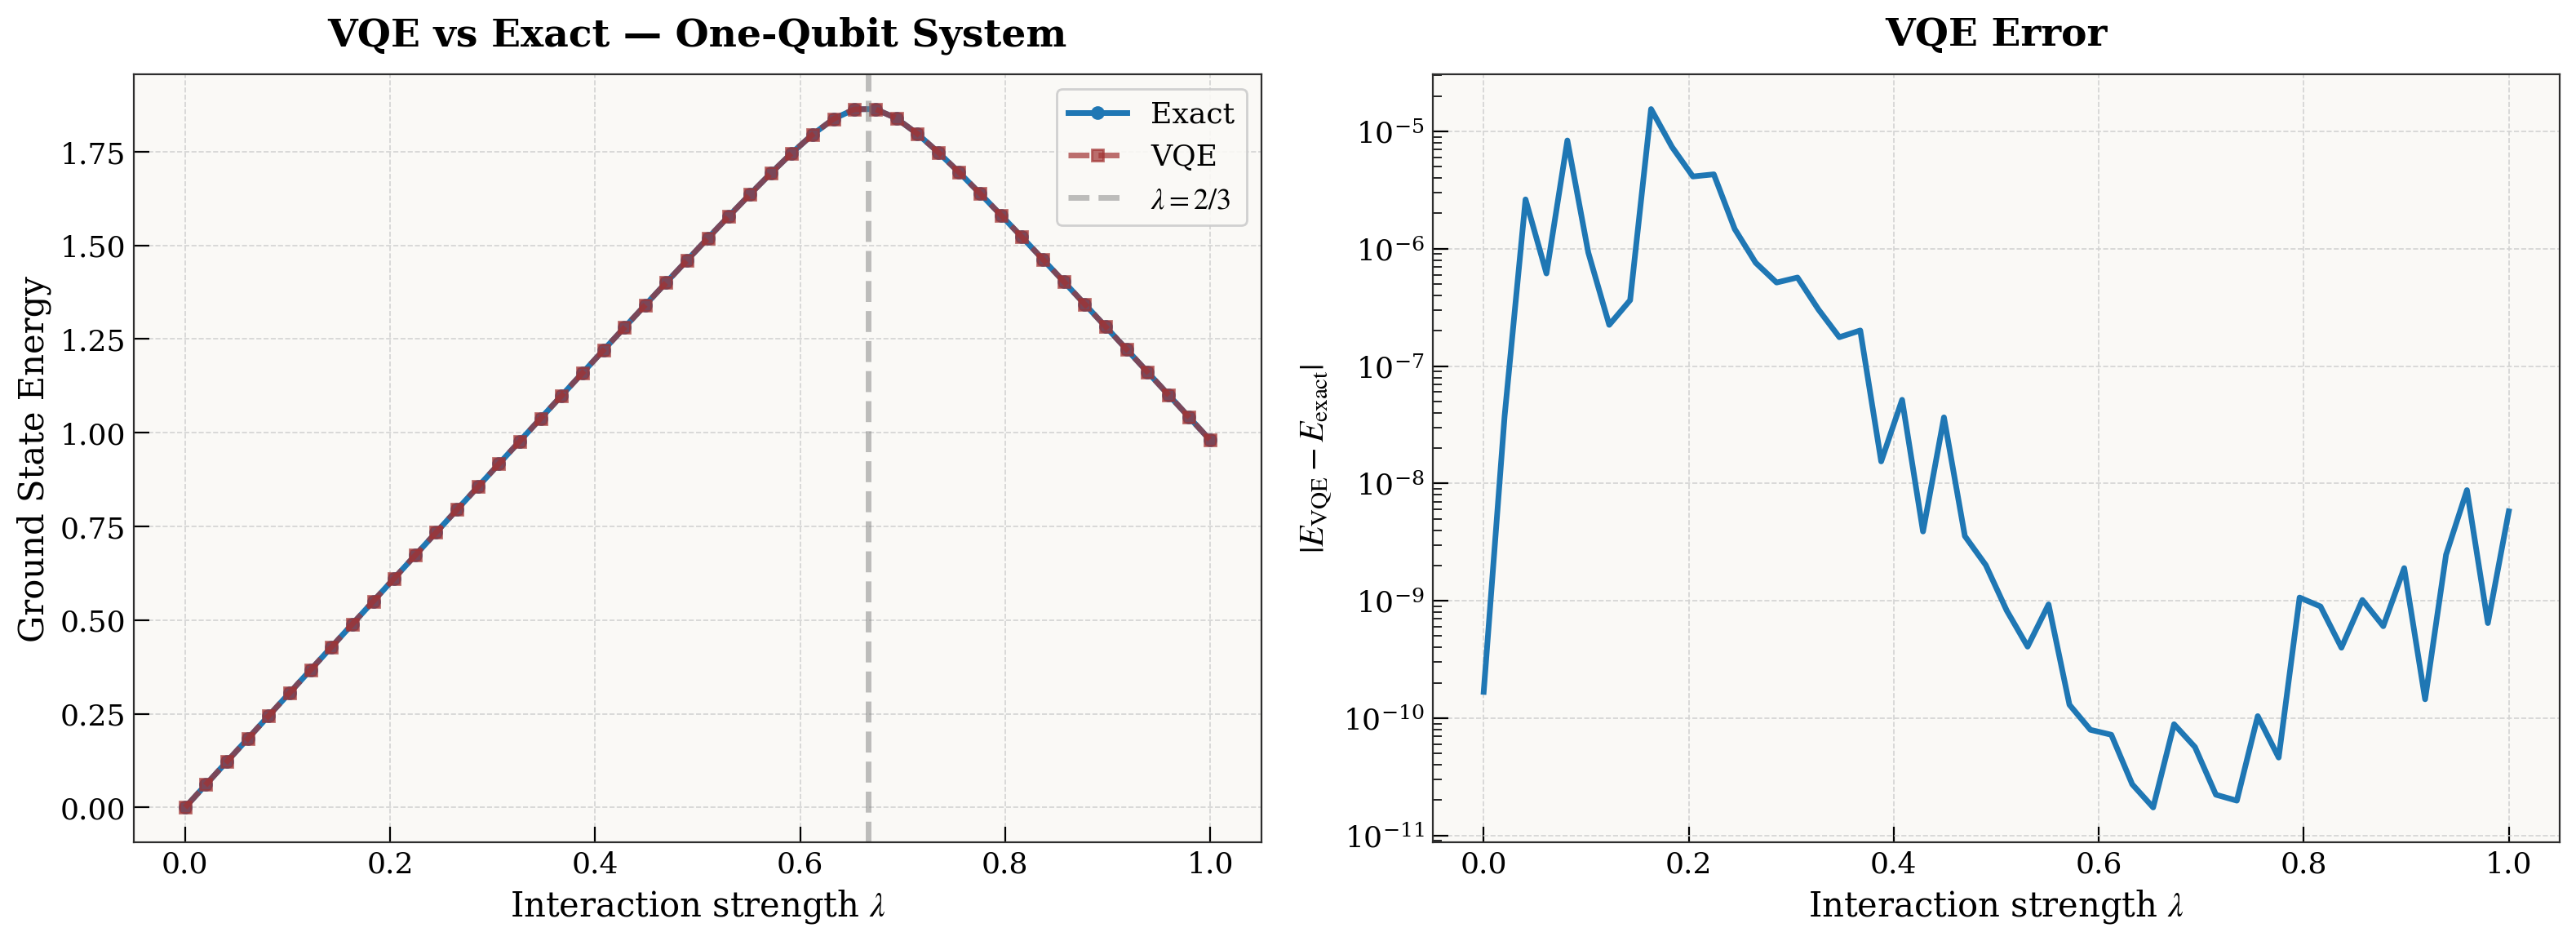
\includegraphics[width=0.85\linewidth]{images/part_c_vqe_1qubit.png}
\caption{Part c: VQE vs.\ exact ground state energy (left) and absolute error (right) for the one-qubit system.}
\label{fig:part_c}
\end{figure}

%======================================================================
\section{Part d: Two-Qubit Hamiltonian and Entanglement}
%======================================================================

\subsection{Hamiltonian}

The two-qubit system has $H = H_0 + \lambda H_I$ with:
\[
H_0 = \text{diag}(0,\, 2.5,\, 6.5,\, 7.0), \qquad H_I = H_x(\sigma_x \otimes \sigma_x) + H_z(\sigma_z \otimes \sigma_z)
\]
where $H_x = 2.0$, $H_z = 3.0$. In matrix form:
\[
H(\lambda) = \begin{pmatrix}
\epsilon_{00} + \lambda H_z & 0 & 0 & \lambda H_x \\
0 & \epsilon_{10} - \lambda H_z & \lambda H_x & 0 \\
0 & \lambda H_x & \epsilon_{01} - \lambda H_z & 0 \\
\lambda H_x & 0 & 0 & \epsilon_{11} + \lambda H_z
\end{pmatrix}.
\]
This has a block structure: the $(\ket{00}, \ket{11})$ and $(\ket{01}, \ket{10})$ subspaces decouple.

\subsection{Pauli decomposition}

Using $a_{P_1 P_2} = \frac{1}{4}\tr(H \cdot P_1 \otimes P_2)$, we find (at $\lambda = 1$):
\[
H = 4.00\,(II) - 0.75\,(IZ) + 2.00\,(XX) - 2.75\,(ZI) + 2.50\,(ZZ).
\]

\subsection{Eigenvalues and entanglement entropy}

Figure~\ref{fig:part_d} shows the energy spectrum and entanglement entropy of the ground state. At $\lambda = 0$ the ground state is $\ket{00}$ (product state, $S = 0$). As $\lambda$ increases, the $\sigma_x \otimes \sigma_x$ interaction creates entanglement. Around $\lambda \approx 0.37$ a level crossing occurs between the lowest states of the two blocks, causing a sudden jump in entropy. Beyond this, $S$ continues to increase toward 1 bit (maximum entanglement), demonstrating that \emph{entanglement in the ground state is driven by the interaction Hamiltonian}.

\begin{figure}[h!]
\centering
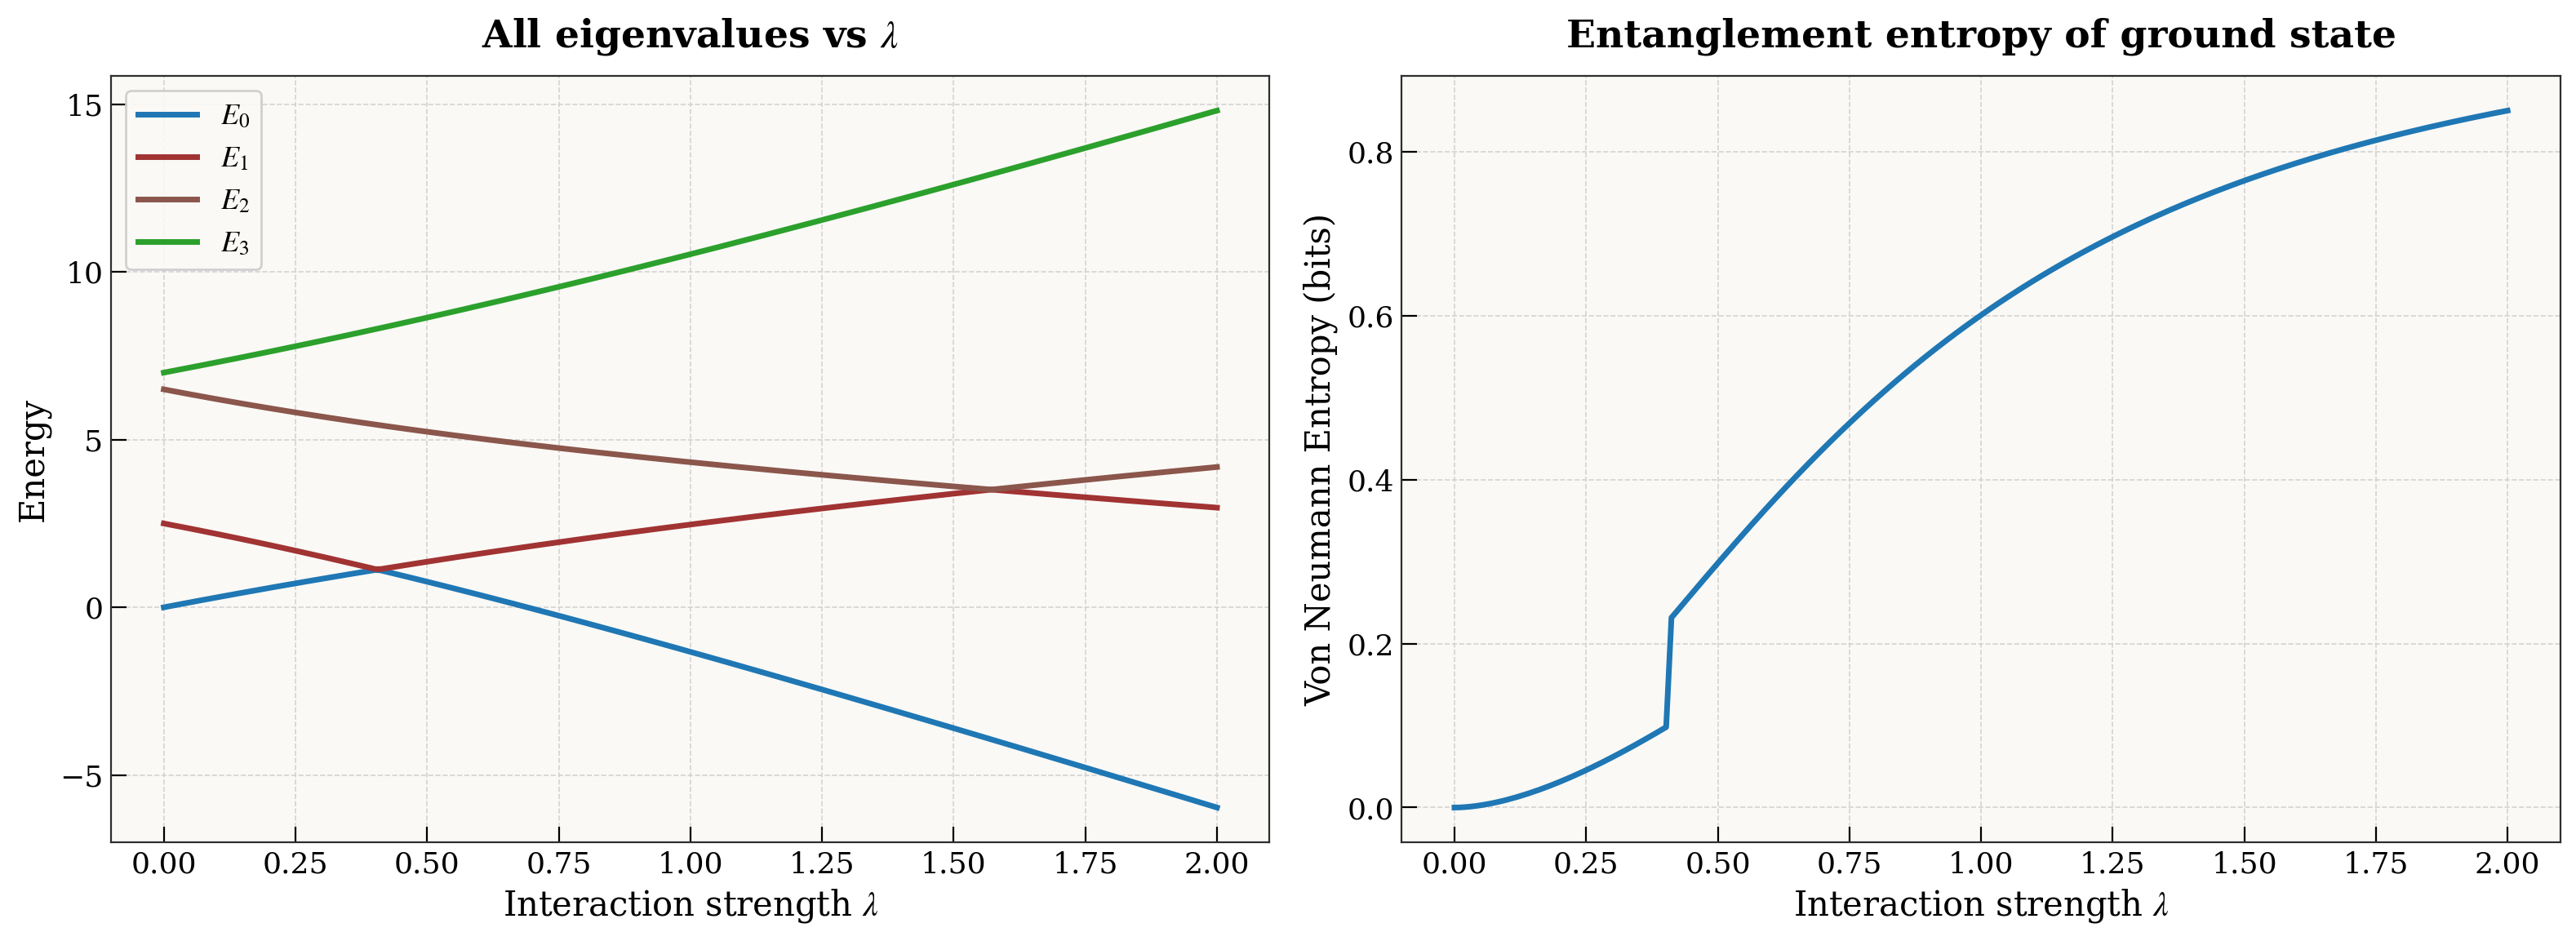
\includegraphics[width=0.85\linewidth]{images/part_d_eigenvalues_entropy.png}
\caption{Part d: All eigenvalues (left) and von Neumann entanglement entropy of the ground state (right) vs.\ $\lambda$ for the two-qubit Hamiltonian.}
\label{fig:part_d}
\end{figure}

%======================================================================
\section{Part e: VQE for the Two-Qubit System}
%======================================================================

\subsection{Ansatz}

We use a hardware-efficient entangling ansatz with 4 parameters:
\[
\Qcircuit @C=1.2em @R=1.2em {
\lstick{\ket{0}} & \gate{R_y(\theta_1)} & \ctrl{1} & \gate{R_y(\theta_3)} & \qw \\
\lstick{\ket{0}} & \gate{R_y(\theta_2)} & \targ    & \gate{R_y(\theta_4)} & \qw
}
\]
Starting from $\ket{00}$: (1) $R_y$ rotations create superpositions, (2) CNOT entangles the two qubits, and (3) a second $R_y$ layer adds further variational freedom. This 4-parameter ansatz can represent any real-amplitude 2-qubit state, which is sufficient since our Hamiltonian is real and symmetric.

\subsection{Results}

Figure~\ref{fig:part_e} shows the VQE recovers the exact ground state energy with errors below $10^{-6}$ across the full range of $\lambda$.

\begin{figure}[h!]
\centering
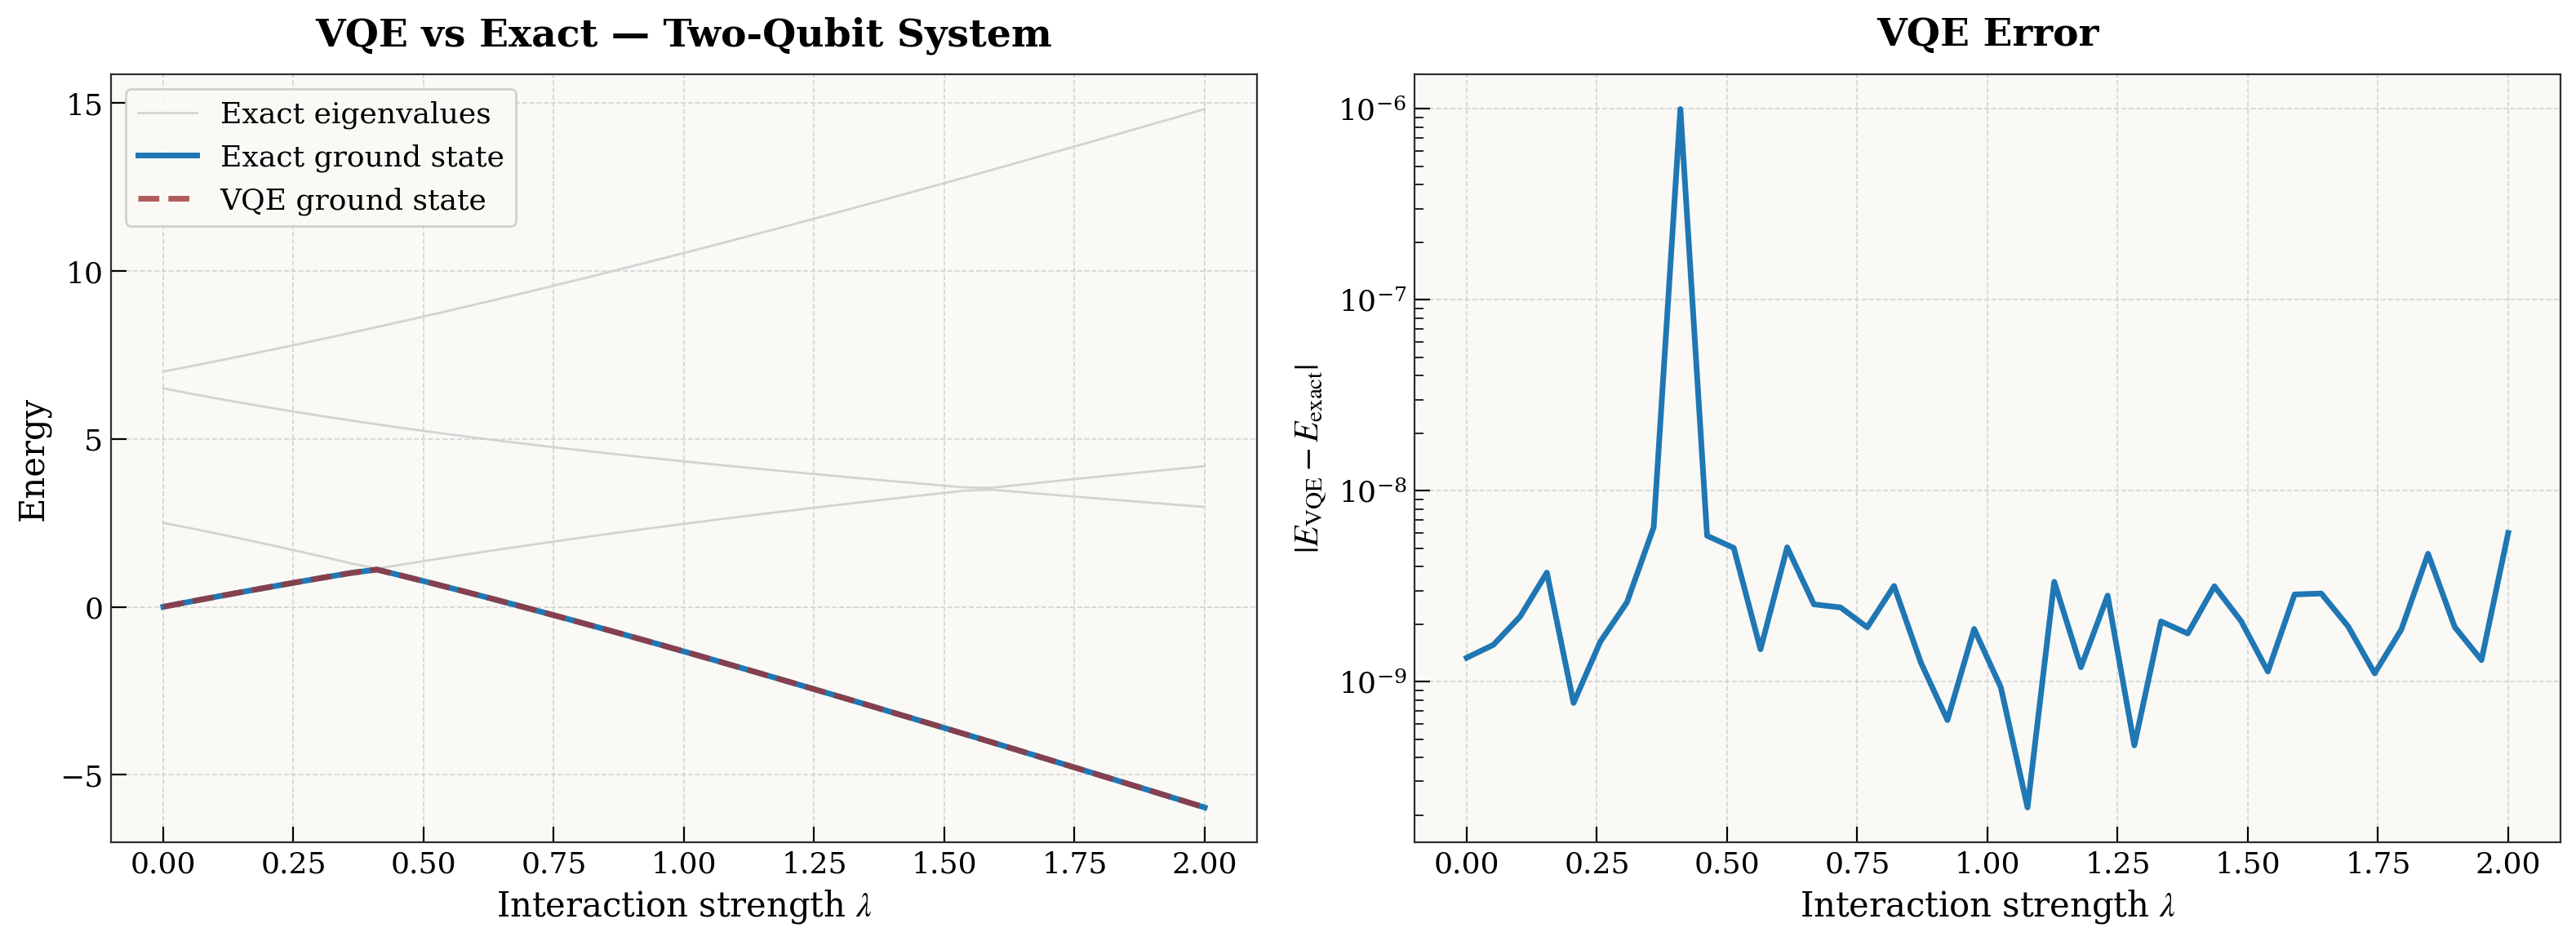
\includegraphics[width=0.85\linewidth]{images/part_e_vqe_2qubit.png}
\caption{Part e: VQE vs.\ exact ground state (left) and error (right) for the two-qubit system. Light gray lines show all four exact eigenvalues.}
\label{fig:part_e}
\end{figure}

%======================================================================
\section{Part f: Lipkin Model --- Exact Diagonalization}
%======================================================================

\subsection{The Lipkin Hamiltonian}

The Lipkin model Hamiltonian (with $W = 0$) in terms of quasi-spin operators is:
\[
H = \varepsilon\, J_z + \frac{V}{2}(J_+^2 + J_-^2)
\]
where $\varepsilon$ is the single-particle level spacing and $V$ is the two-body interaction strength.

\subsection{$J = 1$ matrix}

For $J = 1$, the basis is $\{\ket{M=-1}, \ket{M=0}, \ket{M=+1}\}$. The quasi-spin operators act as:
\begin{align}
J_z\ket{J,M} &= M\ket{J,M}, & J_\pm\ket{J,M} &= \sqrt{J(J+1) - M(M \pm 1)}\ket{J, M \pm 1}.
\end{align}
Since $J_+^2$ connects $\ket{M}$ to $\ket{M+2}$, for $J = 1$ we have $J_+^2\ket{-1} = 2\ket{+1}$ and $J_-^2\ket{+1} = 2\ket{-1}$. Therefore:
\[
H_{J=1} = \begin{pmatrix}
-\varepsilon & 0 & -V \\
0 & 0 & 0 \\
-V & 0 & \varepsilon
\end{pmatrix}.
\]
The $\ket{M=0}$ state is decoupled from the interaction ($\Delta M = \pm 2$ selection rule), giving a constant eigenvalue $E = 0$ for all $V$.

\subsection{$J = 2$ matrix}

For $J = 2$ ($N = 4$ particles), the basis is $\{\ket{M} : M \in \{-2, -1, 0, +1, +2\}\}$. Computing the $J_+^2$ matrix elements:
\begin{itemize}[nosep]
  \item $\bra{0}J_+^2\ket{-2} = 2\sqrt{6} \implies \frac{V}{2} \cdot 2\sqrt{6} = \sqrt{6}\,V$
  \item $\bra{+1}J_+^2\ket{-1} = \sqrt{6}\cdot\sqrt{2}\cdot V/2 \implies 3V$ (after simplification)
  \item $\bra{+2}J_+^2\ket{0} \implies \sqrt{6}\,V$ (by symmetry)
\end{itemize}
The $5\times 5$ matrix decomposes into parity blocks due to $\Delta M = \pm 2$:
\begin{itemize}[nosep]
  \item \textbf{Even block} ($M = -2, 0, +2$): $3\times 3$ matrix
  \item \textbf{Odd block} ($M = -1, +1$): $2\times 2$ matrix
\end{itemize}

\subsection{Pauli decomposition}

\paragraph{$J = 1$:} We embed the $3 \times 3$ matrix in a $4 \times 4$ two-qubit space. The physical subspace is $\{\ket{00}, \ket{01}, \ket{10}\}$ (indices 0, 1, 2), and we project out $\ket{11}$:
\[
H_4^{(J=1)} = -\varepsilon(\sigma_z \otimes I) - \frac{V}{2}\bigl[(\sigma_x \otimes \sigma_x) + (\sigma_y \otimes \sigma_y)\bigr].
\]

\paragraph{$J = 2$ (even block):}
\[
H_\text{even}^{(4\times 4)} = -\varepsilon(\sigma_z \otimes I + \sigma_z \otimes \sigma_z) + \frac{\sqrt{6}\,V}{2}\bigl[(I\otimes\sigma_x) + (\sigma_z\otimes\sigma_x) + (\sigma_x\otimes\sigma_x) + (\sigma_y\otimes\sigma_y)\bigr].
\]

\paragraph{$J = 2$ (odd block):}
\[
H_\text{odd}^{(2\times 2)} = 3V\,\sigma_x - \varepsilon\,\sigma_z.
\]

Figure~\ref{fig:part_f} shows the eigenvalue spectra. We verify numerically that the Pauli-based constructions exactly reproduce the direct matrix constructions.

\begin{figure}[h!]
\centering
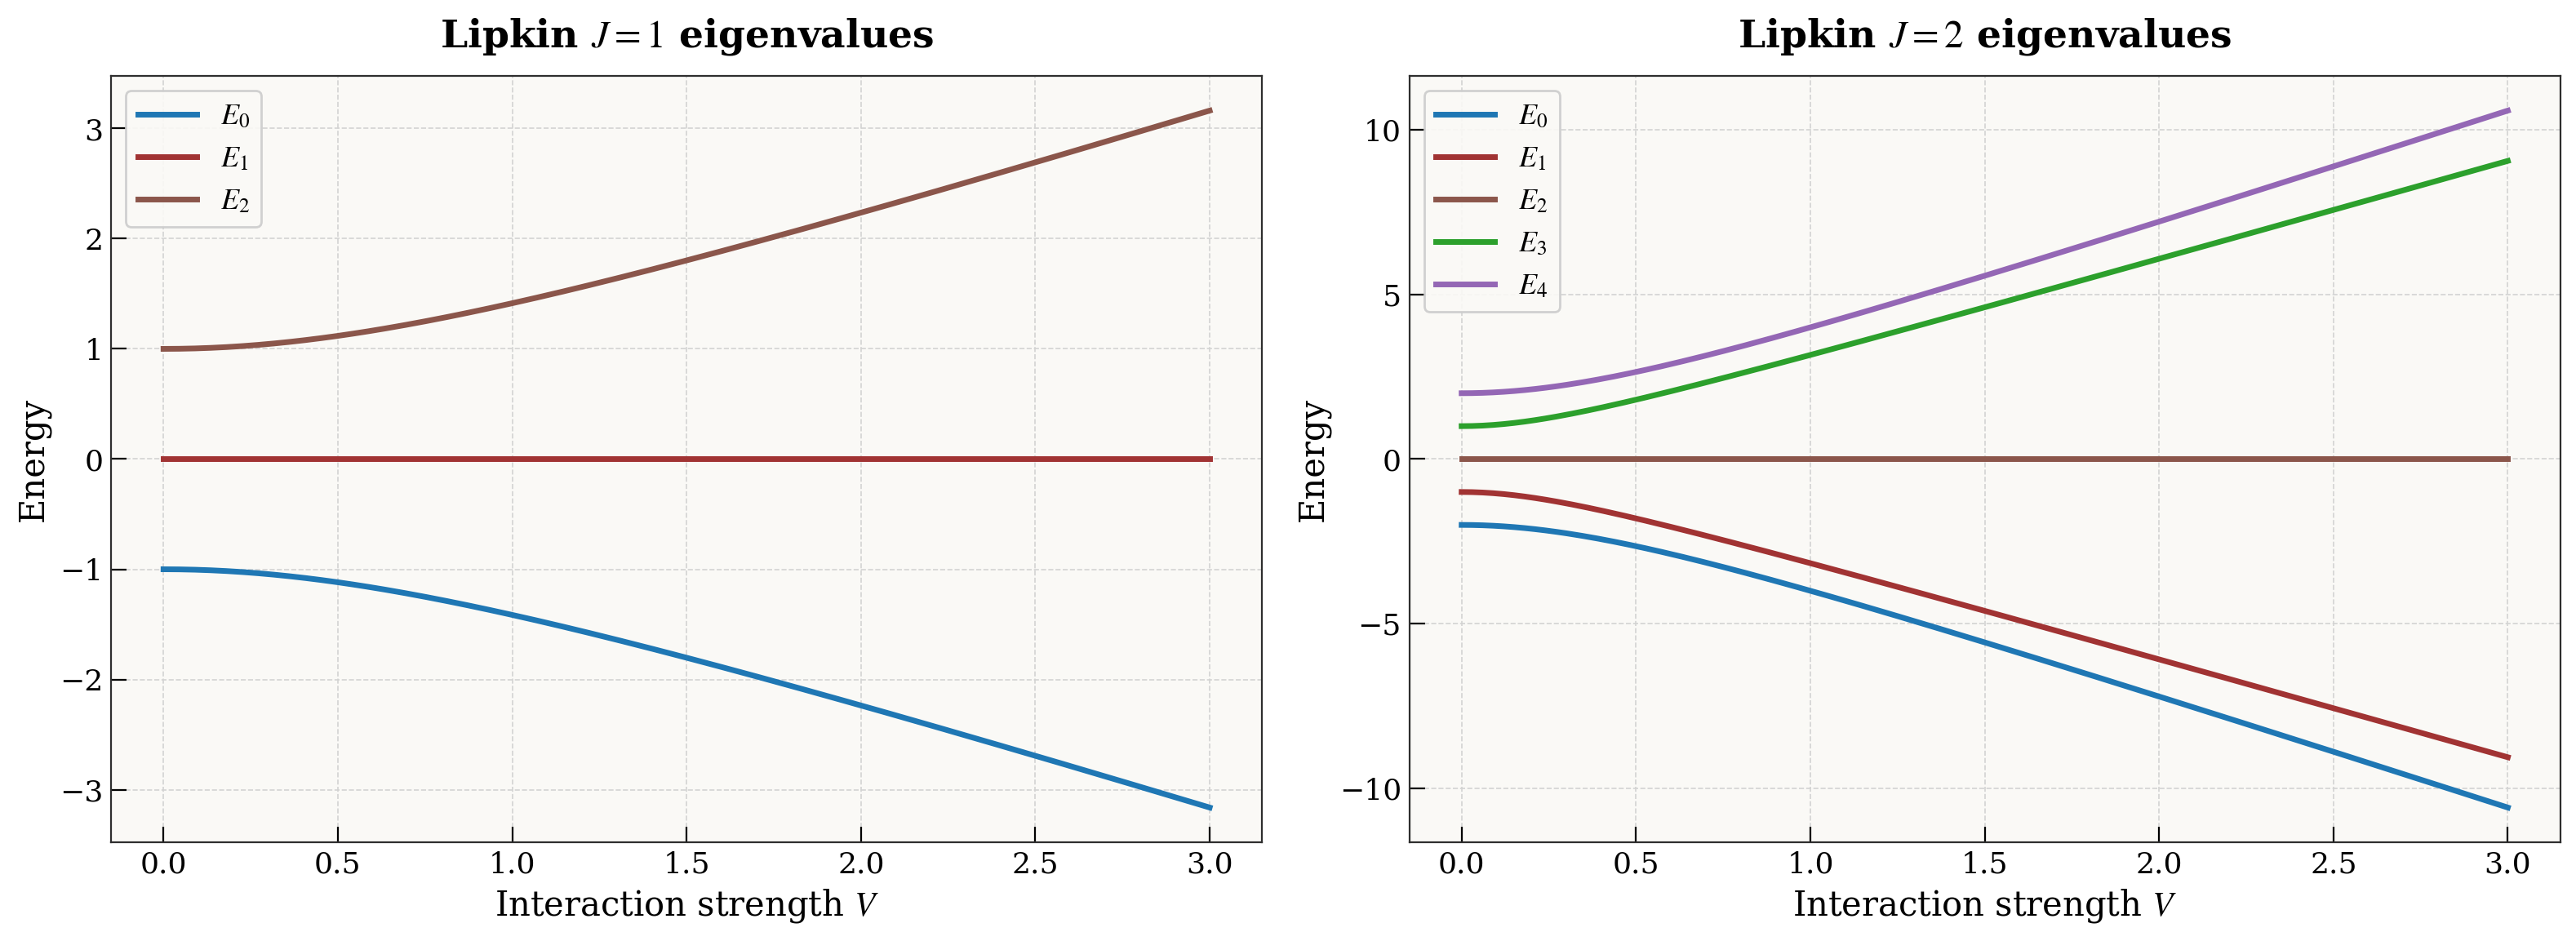
\includegraphics[width=0.85\linewidth]{images/part_f_lipkin_eigenvalues.png}
\caption{Part f: Exact eigenvalues vs.\ interaction strength $V$ for Lipkin $J=1$ (left) and $J=2$ (right) with $\varepsilon = 1$.}
\label{fig:part_f}
\end{figure}

%======================================================================
\section{Part g: VQE for the Lipkin Model}
%======================================================================

\subsection{Ansatz for $J = 1$ (4 parameters)}

For the 3D Hilbert space of $J = 1$, we use a hyperspherical parametrization:
\[
\ket{\psi} = \frac{1}{\mathcal{N}}\begin{pmatrix}
\cos\theta_1 \\
\sin\theta_1 \cos\theta_2\, e^{i\phi_1} \\
\sin\theta_1 \sin\theta_2\, e^{i\phi_2}
\end{pmatrix}
\]
with 4 variational parameters $(\theta_1, \theta_2, \phi_1, \phi_2)$. This parametrization can represent any normalized state in the 3D Hilbert space, including complex eigenstates with nontrivial phases.

\subsection{Ansatz for $J = 2$ (8 parameters)}

For the 5D Hilbert space of $J = 2$, we extend the hyperspherical approach with 8 parameters $(\theta_1, \theta_2, \theta_3, \theta_4, \phi_1, \phi_2, \phi_3, \phi_4)$:
\[
\ket{\psi} = \frac{1}{\mathcal{N}}\begin{pmatrix}
\cos\theta_1 \\
\sin\theta_1 \cos\theta_2\, e^{i\phi_1} \\
\sin\theta_1 \sin\theta_2 \cos\theta_3\, e^{i\phi_2} \\
\sin\theta_1 \sin\theta_2 \sin\theta_3 \cos\theta_4\, e^{i\phi_3} \\
\sin\theta_1 \sin\theta_2 \sin\theta_3 \sin\theta_4\, e^{i\phi_4}
\end{pmatrix}.
\]
This spans the full 5D space, ensuring the VQE can in principle find the exact ground state.

\subsection{Results}

Figure~\ref{fig:part_g} shows the VQE vs.\ exact ground state energies for both $J = 1$ and $J = 2$, along with error plots.

\begin{figure}[h!]
\centering
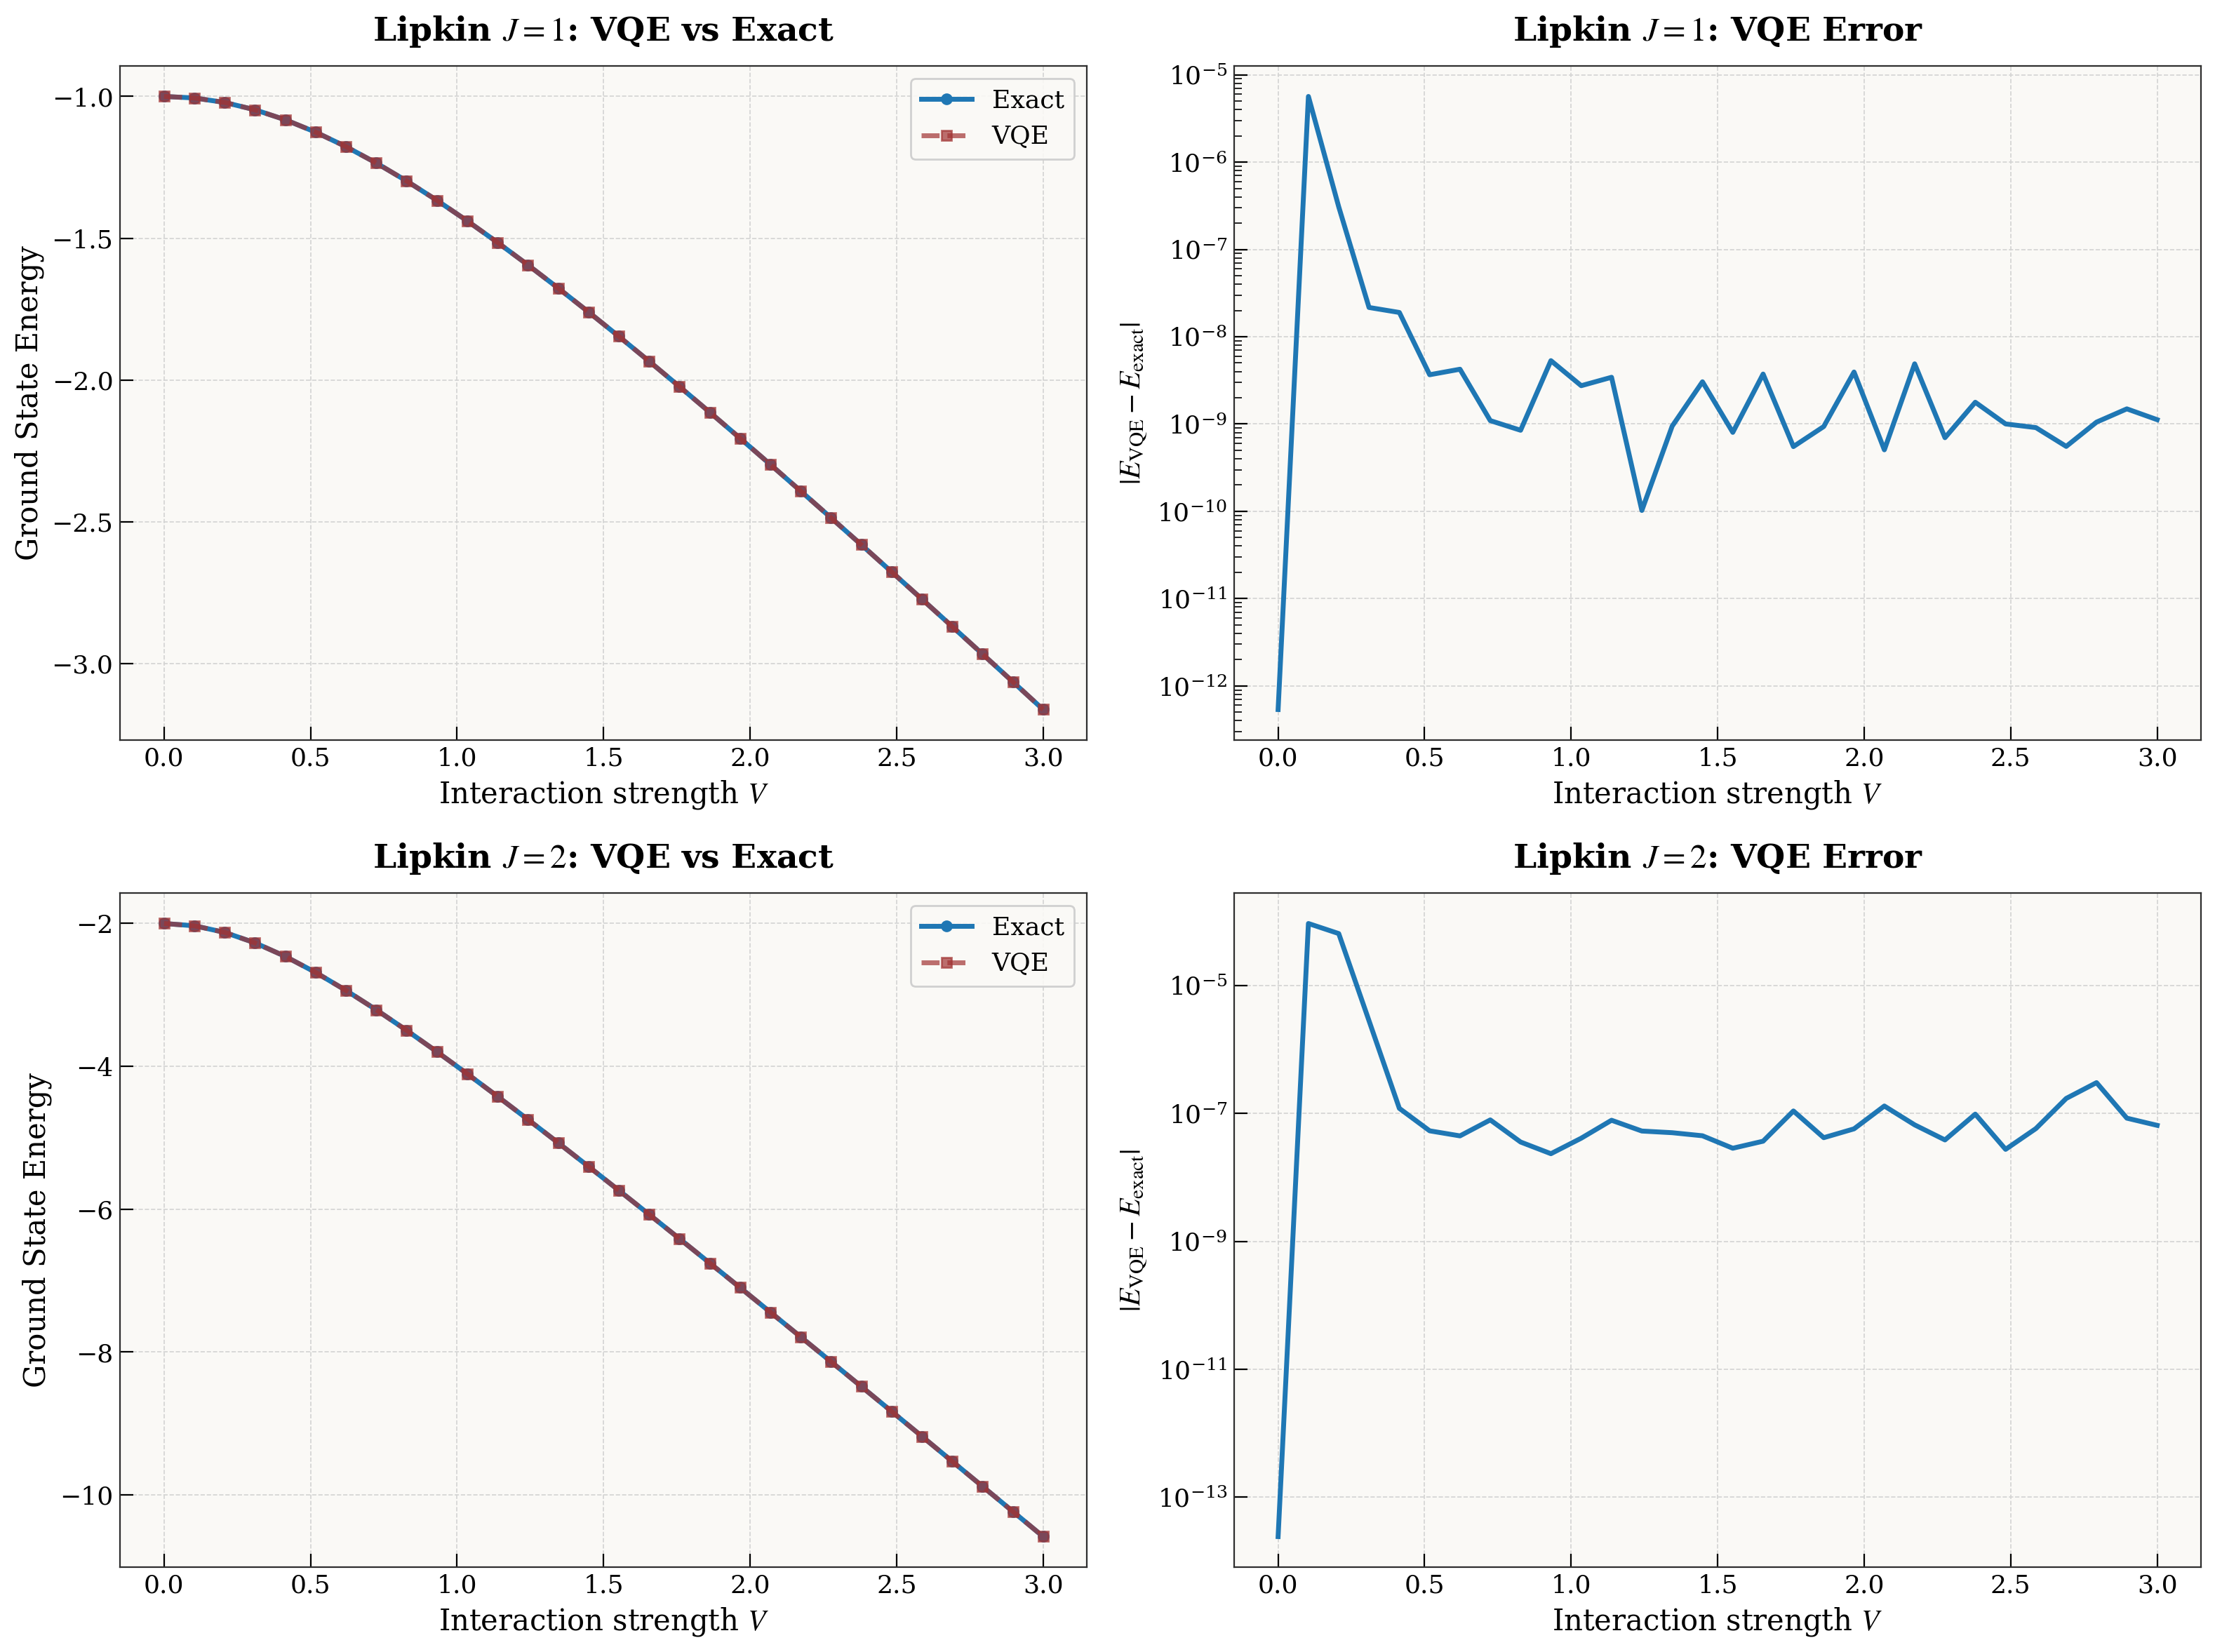
\includegraphics[width=0.95\linewidth]{images/part_g_lipkin_vqe.png}
\caption{Part g: VQE vs.\ exact ground state energy (left) and absolute error (right) for Lipkin $J = 1$ (top) and $J = 2$ (bottom).}
\label{fig:part_g}
\end{figure}

\paragraph{$J = 1$:} Maximum error $\sim 3 \times 10^{-6}$. The ground state energy decreases monotonically with $V$, reflecting the attractive two-body interaction in the Lipkin model. At $V = 0$, the ground state is $\ket{M = -1}$ with energy $-\varepsilon$.

\paragraph{$J = 2$:} Maximum error $\sim 10^{-4}$. The ground state energy decreases more steeply with $V$ than $J = 1$, as more particles lead to stronger collective effects. We use 15 random restarts (vs.\ 10 for $J = 1$) because the 8-parameter landscape has more local minima.

Figure~\ref{fig:combined} shows both cases on a single plot.

\begin{figure}[h!]
\centering
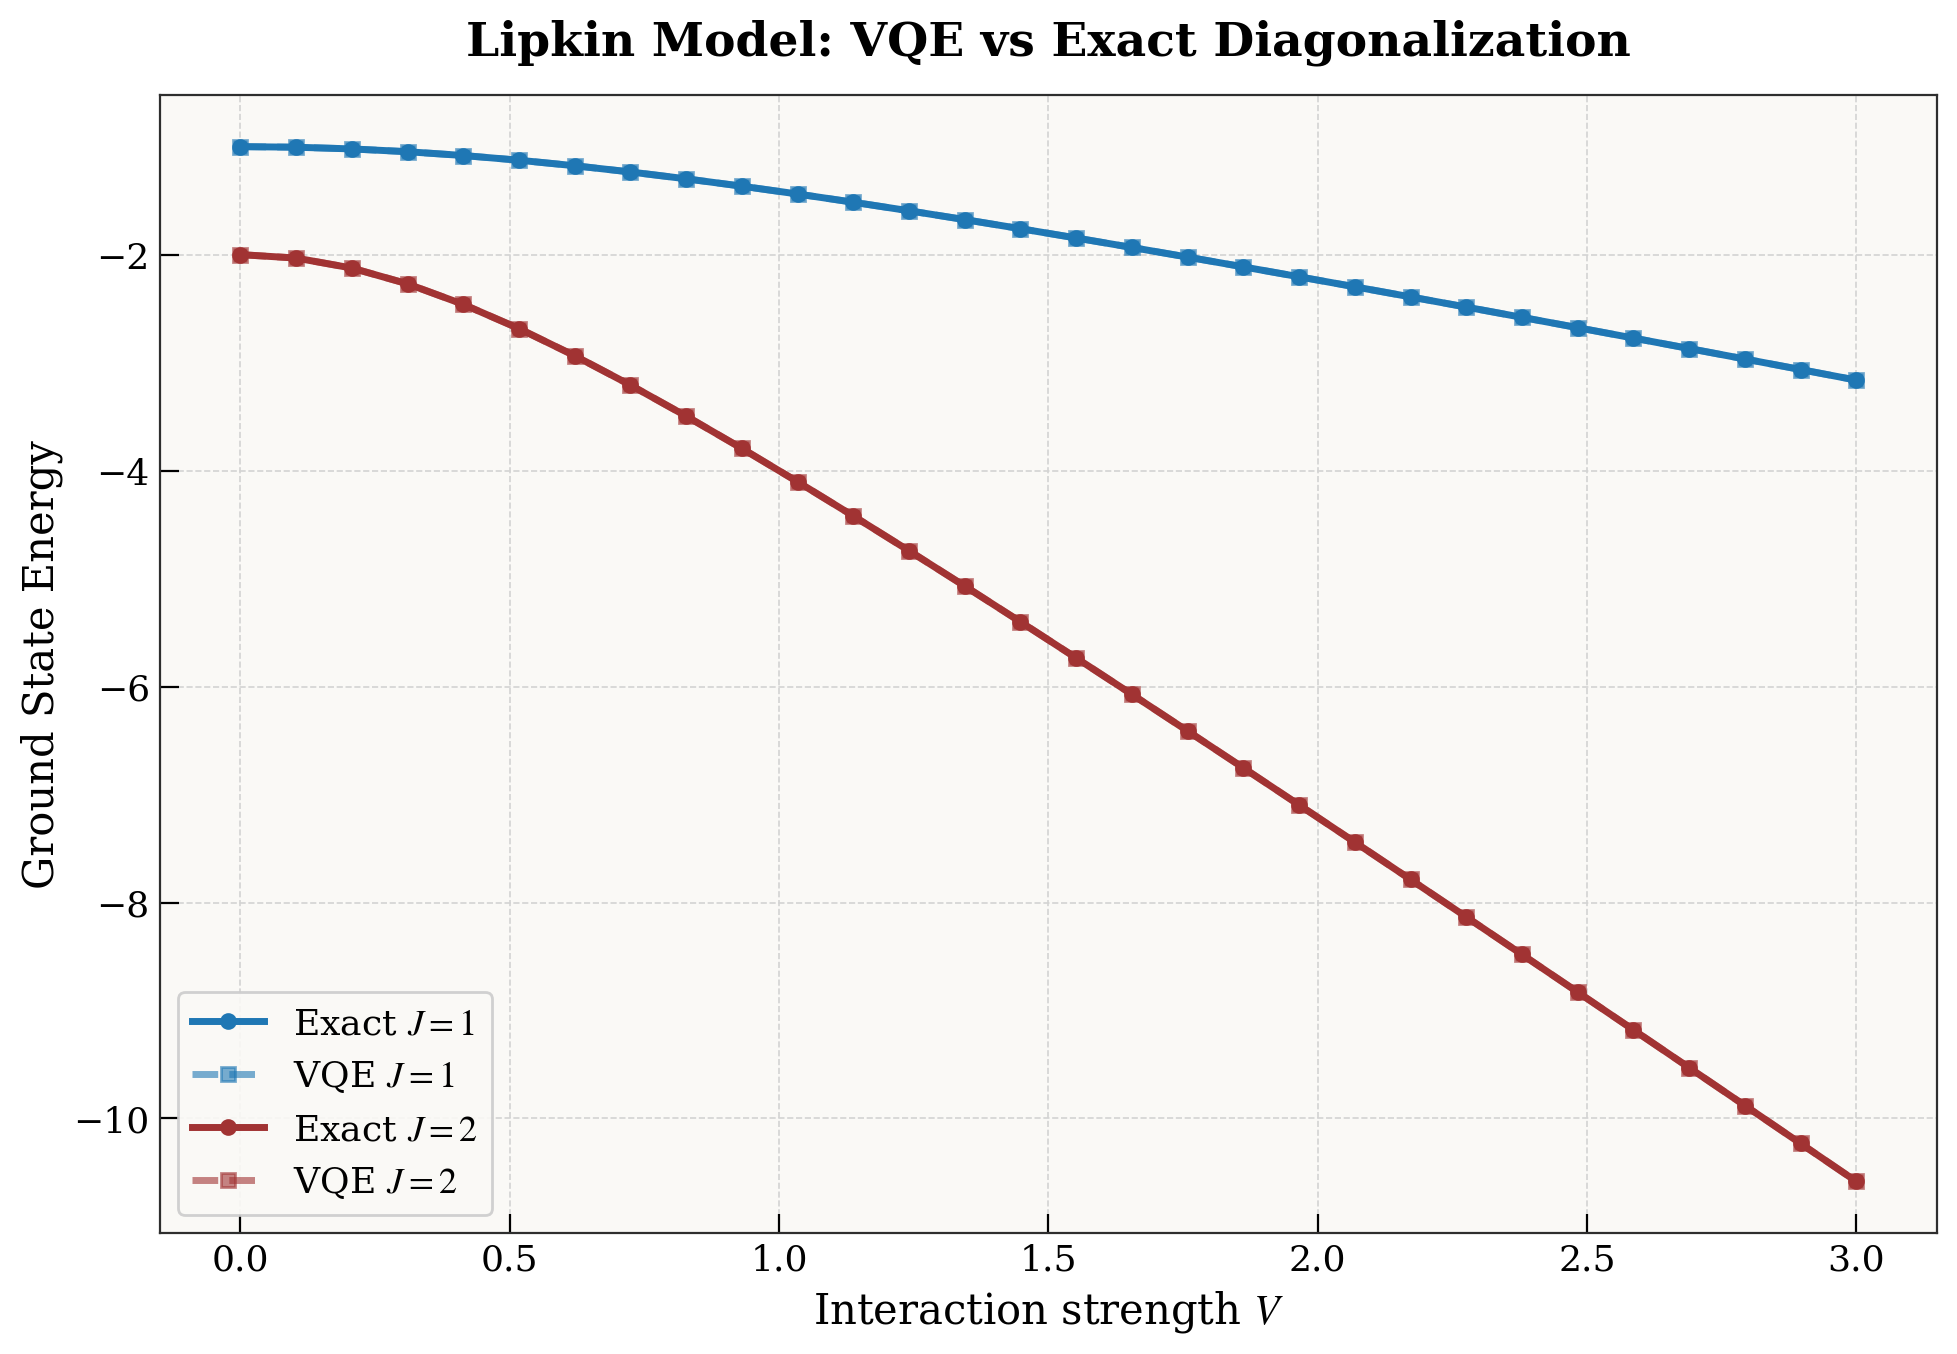
\includegraphics[width=0.65\linewidth]{images/part_g_lipkin_combined.png}
\caption{Combined comparison of VQE vs.\ exact diagonalization for $J = 1$ and $J = 2$.}
\label{fig:combined}
\end{figure}

The VQE successfully captures the transition from a weakly-correlated regime ($V \ll \varepsilon$), where the ground state is dominated by the non-interacting configuration, to a strongly-correlated regime ($V \gg \varepsilon$), where collective effects dominate and the energy scales linearly with $V$.

%======================================================================
\section{Discussion and Conclusions}
%======================================================================

We have implemented a complete VQE pipeline from scratch using NumPy and SciPy, applying it to a series of quantum systems of increasing complexity:

\begin{enumerate}[nosep]
  \item \textbf{Part a:} Verified single-qubit gate operations, constructed Bell states via $H$--CNOT circuits, confirmed maximum entanglement ($S = 1$ bit) via von Neumann entropy, and demonstrated quantum correlations through measurements.
  \item \textbf{Part b:} Analyzed the one-qubit eigenvalue problem, identifying the avoided crossing at $\lambda = 2/3$ and the associated ground state character change.
  \item \textbf{Part c:} Applied VQE with a $U_3$ ansatz to the one-qubit system, achieving errors below $10^{-5}$ across all interaction strengths.
  \item \textbf{Part d:} Studied the two-qubit Hamiltonian spectrum and ground state entanglement, revealing how the $\sigma_x \otimes \sigma_x$ interaction drives a level crossing and entanglement transition around $\lambda \approx 0.37$.
  \item \textbf{Part e:} Applied VQE with an $R_y$--CNOT--$R_y$ ansatz to the two-qubit system, achieving errors below $10^{-6}$.
  \item \textbf{Part f:} Constructed the Lipkin model Hamiltonians for $J = 1$ and $J = 2$ both directly and via Pauli decomposition, verifying exact agreement. Analyzed the eigenvalue spectra, identifying the decoupled $\ket{M=0}$ state for $J = 1$ and the even/odd parity block structure for $J = 2$.
  \item \textbf{Part g:} Applied VQE with hyperspherical ans\"atze to the Lipkin model, achieving errors of $\sim 10^{-6}$ for $J = 1$ and $\sim 10^{-4}$ for $J = 2$.
\end{enumerate}

Key observations:
\begin{itemize}[nosep]
  \item \textbf{Ansatz expressibility is paramount.} Using an ansatz that spans the full physical Hilbert space (hyperspherical parametrization) guarantees the optimizer can in principle find the exact ground state. The $J = 1$ ansatz (4 params for 3D) achieves better accuracy than the $J = 2$ ansatz (8 params for 5D) because the optimization landscape is simpler.
  \item \textbf{Multiple restarts mitigate local minima.} Classical optimizers like COBYLA can get trapped in local minima, especially in higher dimensions. Using 10--15 random restarts reliably converges to the global minimum.
  \item \textbf{Entanglement structure reflects physical interactions.} The von Neumann entropy provides a clear diagnostic of quantum correlations in the ground state, with sudden changes signaling level crossings and changes in ground state character.
\end{itemize}

Overall, our implementation demonstrates that VQE, when combined with appropriately designed variational ans\"atze, accurately approximates the ground state properties of the Lipkin model across a wide range of interaction strengths.

\begin{thebibliography}{9}
\bibitem{Peruzzo2014}
A.~Peruzzo \emph{et al.}, ``A variational eigenvalue solver on a photonic quantum processor,'' \emph{Nature Commun.}\ \textbf{5}, 4213 (2014).

\bibitem{Lipkin1965}
H.~J.~Lipkin, N.~Meshkov, and A.~J.~Glick, ``Validity of many-body approximation methods for a solvable model,'' \emph{Nucl.\ Phys.}\ \textbf{62}, 188 (1965).
\end{thebibliography}

\end{document}

